\documentclass{standalone}
\usepackage{tikz}
\usepackage{ctex,siunitx}
\usepackage{tkz-euclide}
\usepackage{amsmath}
\usetikzlibrary{patterns, calc}
\usetikzlibrary {decorations.pathmorphing, decorations.pathreplacing, decorations.shapes,}
\begin{document}
\small
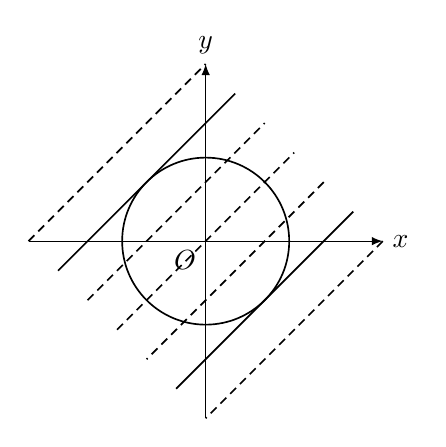
\begin{tikzpicture}[>=latex,scale=0.75,samples=200]
  % \useasboundingbox(0,-0.2)rectangle(3,0.5);
  \draw[thin,->](-3,0)--(3,0)node[right]{$x$};
  \draw[thin,->](0,-3)--(0,3)node[above]{$y$};
  \tkzDefPoints{0/0/O}
  \draw[semithick](0,0)circle({sqrt(2)});
  \draw[semithick](-2.5,-0.5)--(0.5,2.5);
  \draw[semithick](2.5,0.5)--(-0.5,-2.5);
  \draw[semithick,densely dashed](-3,0)--(0,3);
  \draw[semithick,densely dashed](-2,-1)--(1,2);
  \draw[semithick,densely dashed](-1.5,-1.5)--(1.5,1.5);
  \draw[semithick,densely dashed](2,1)--(-1,-2);
  \draw[semithick,densely dashed](3,0)--(0,-3);
  \tkzLabelPoints[below left](O)
\end{tikzpicture}
\end{document}